\documentclass[10pt]{article}
\usepackage[utf8]{inputenc}
\usepackage{listings}
\usepackage{float}
\usepackage{graphicx}
\usepackage{fullpage}
\usepackage{caption}
\usepackage{subcaption}
\usepackage{amsmath}
\usepackage{hyperref}

%\renewcommand{\thesubsection}{\arabic{subsection}}
\renewcommand{\thesubsubsection}{\alph{subsubsection}}

\title{Pattern Recognition Practical 5}
\author{Group 24: \and Maikel Withagen (s1867733) \and Steven Bosch (s1861948)}
\date{\today}
\lstset{
frame=single, 
numbers=left, 
breaklines=true, 
language=Matlab,
basicstyle=\footnotesize, 
title=\lstname,
showstringspaces=false
}

\renewcommand{\thesection}{Assignment \arabic{section}}
\renewcommand{\thesubsection}{\arabic{subsection}}
\begin{document}
\maketitle

\section{k-means clustering, quantization error, gap statistic}
\subsection{}
Using the code given in the Appendix(kmeans.m and runKMeans.m), 
we created the plots shown in figures \ref{fig1.1}, \ref{fig1.2} and \ref{fig1.3}.\\

\begin{figure}[H]
  \centering
  \caption{Results for k=2}
  \begin{subfigure}[b]{.45\textwidth}
    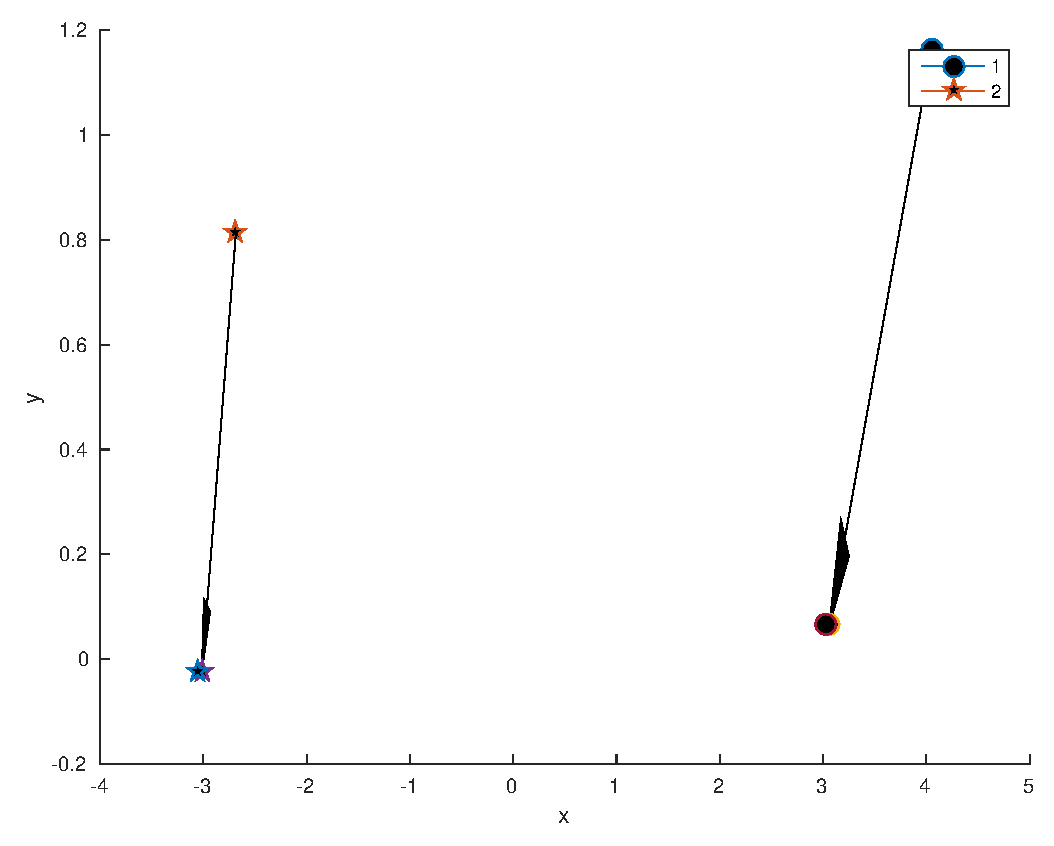
\includegraphics[width=\columnwidth]{Fig1_k2.eps}
    \caption{intermediate positions of the cluster means, 
    with their progress indicated by the arrows.}
    \label{fig1a}
  \end{subfigure}
  \quad
  \begin{subfigure}[b]{.45\textwidth}
    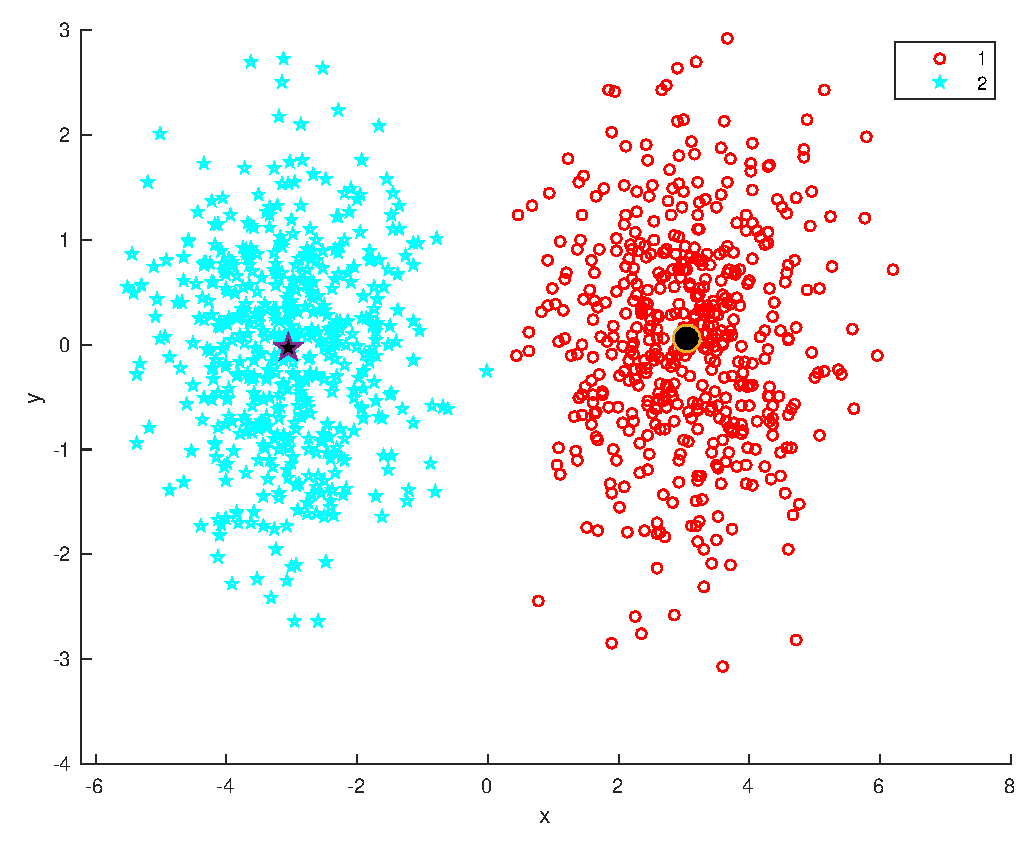
\includegraphics[width=\columnwidth]{Fig2_k2.eps}
    \caption{The final cluster means with their assigned data points)}
    \label{fig1b}
  \end{subfigure}
  \label{fig1.1}
\end{figure}

\begin{figure}[H]
  \centering
  \caption{Results for k=4}
  \begin{subfigure}[b]{.45\textwidth}
    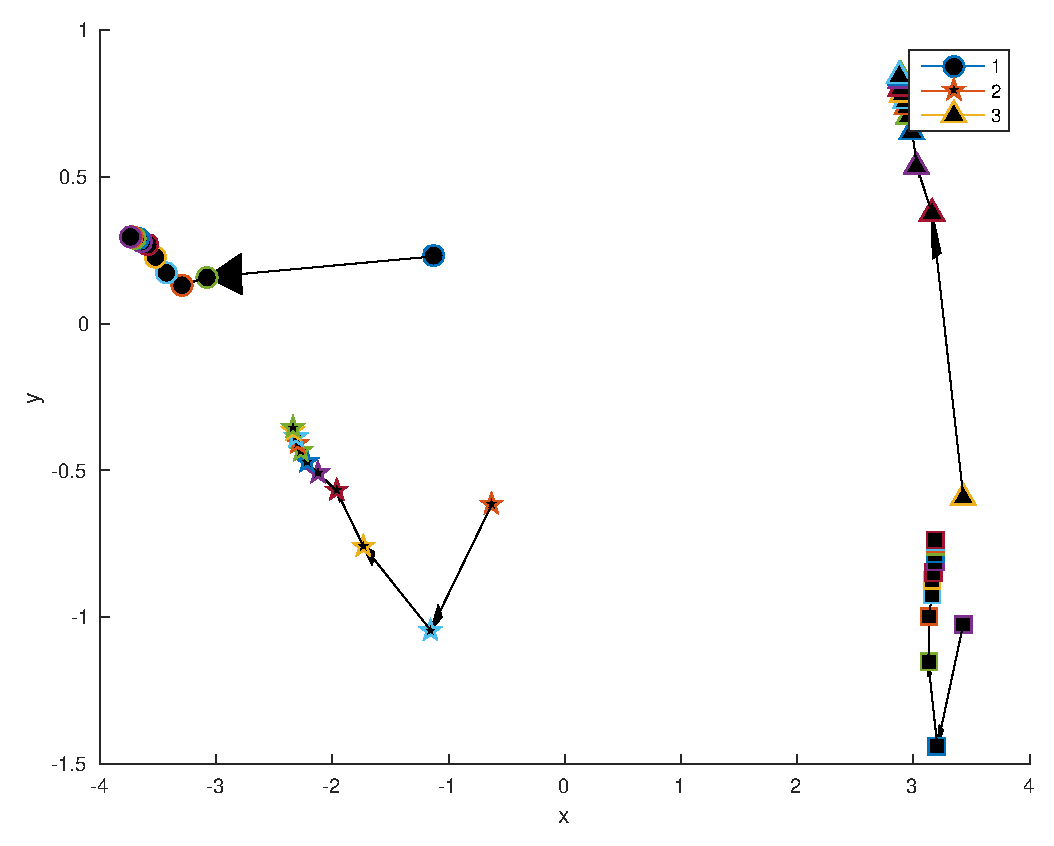
\includegraphics[width=\columnwidth]{Fig1_k4.eps}
    \caption{intermediate positions of the cluster means, 
    with their progress indicated by the arrows.}
  \end{subfigure}
  \quad
  \begin{subfigure}[b]{.45\textwidth}
    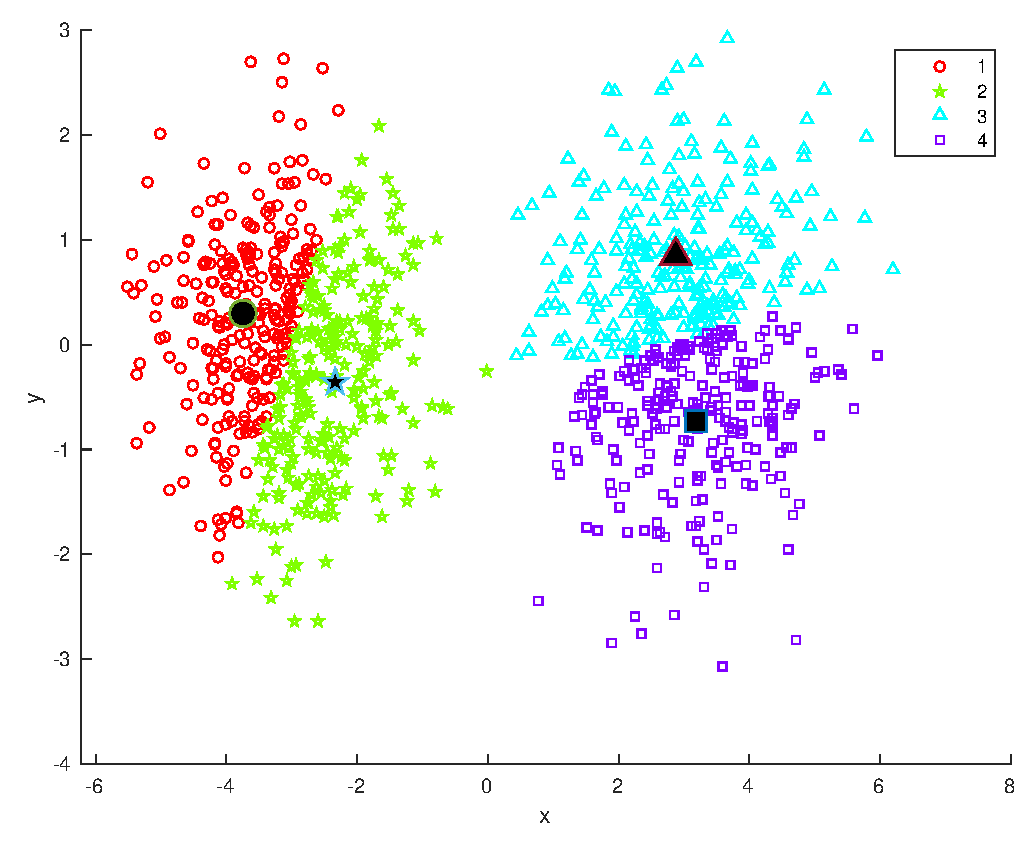
\includegraphics[width=\columnwidth]{Fig2_k4.eps}
    \caption{The final cluster means with their assigned data points)}
  \end{subfigure}
  \label{fig1.2}
\end{figure}

\begin{figure}[H]
  \centering
  \caption{Results for k=8}
  \begin{subfigure}[b]{.45\textwidth}
    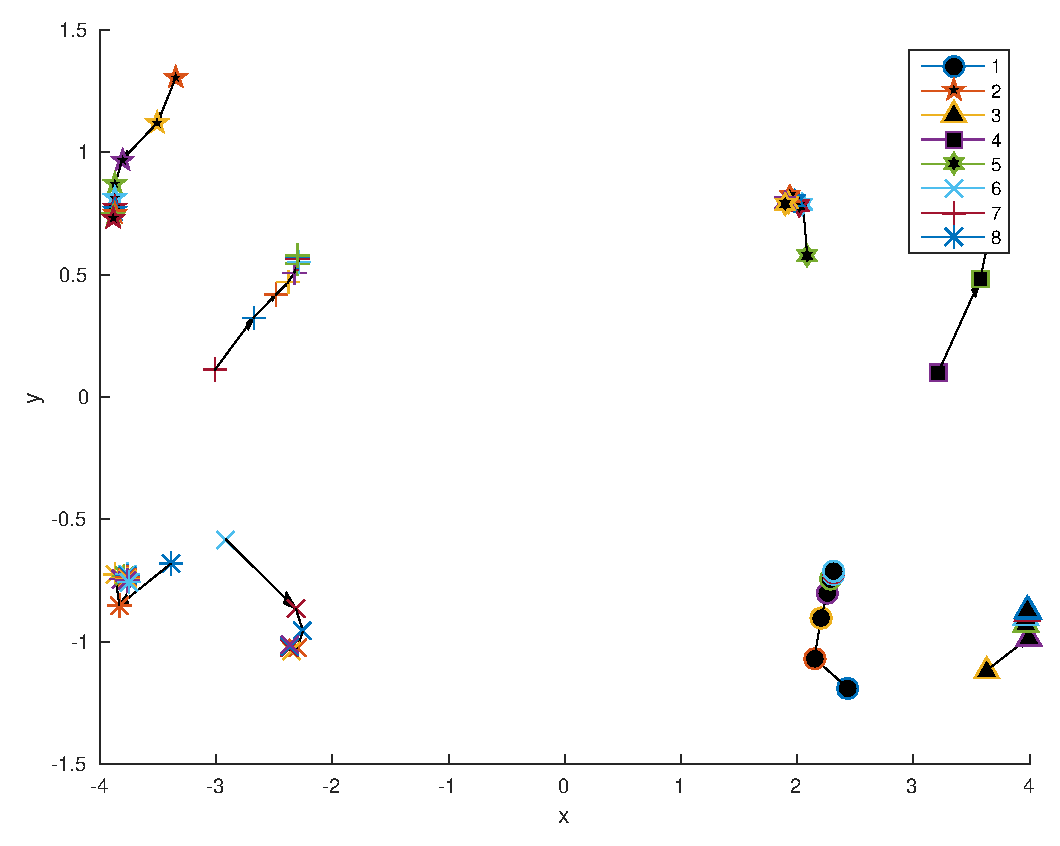
\includegraphics[width=\columnwidth]{Fig1_k8.eps}
    \caption{intermediate positions of the cluster means, 
    with their progress indicated by the arrows.}
  \end{subfigure}
  \quad
  \begin{subfigure}[b]{.45\textwidth}
    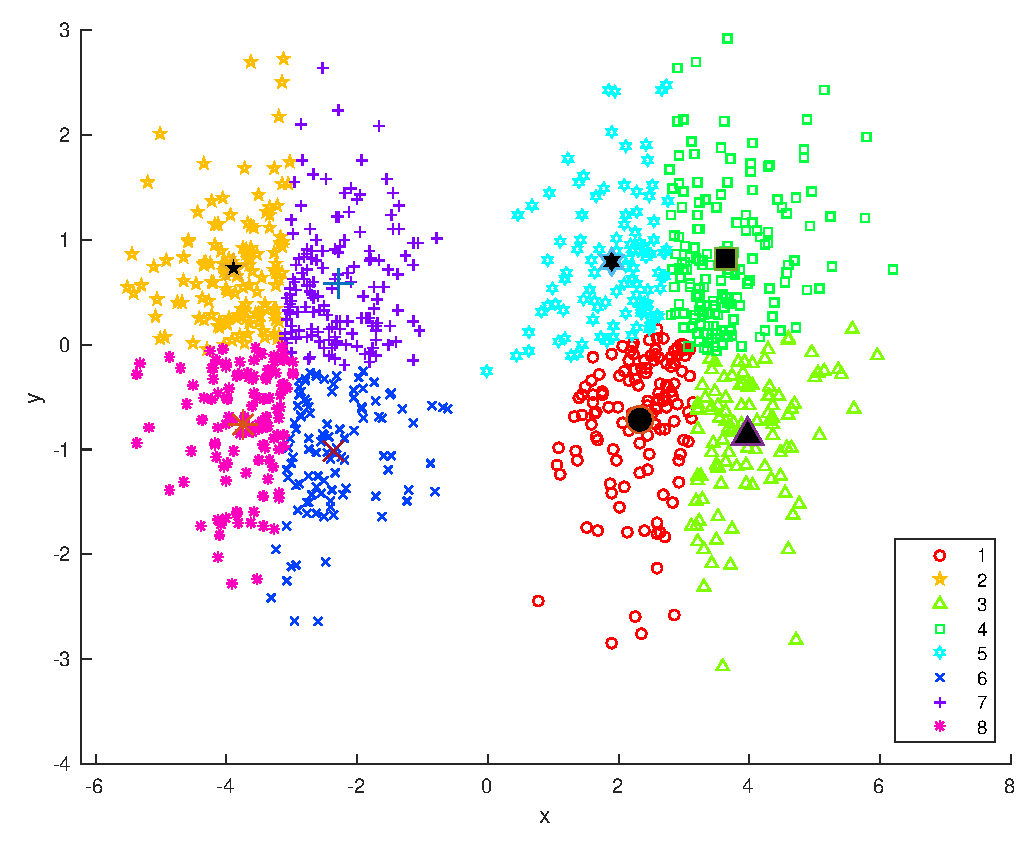
\includegraphics[width=\columnwidth]{Fig2_k8.eps}
    \caption{The final cluster means with their assigned data points)}
  \end{subfigure}
  \label{fig1.3}
\end{figure}

\noindent We we can clearly see that the data form two clusters. Therefore figure \ref{fig1a} shows the quickest convergence to the final cluster centers. Usually it takes about two epochs for the cluster centers to converge, as is shown in the figure. Figure \ref{fig1b} shows that these centers form in the places which the human eye observes to be the correct centers. When we choose k as 4, as shown in figure \ref{fig1.2}, we can see that the two clusters get separated into two clusters each (although this is dependent on the initialization). The number of epochs is quite higher. This can be explained by the fact that the data are not naturally separated into four clusters but in two, so the distances between the data points within a main cluster are small. This causes the algorithm to take longer to find a convergence, since the cluster centers switch often during the clustering process. Finally figure \ref{fig1.3} shows the clustering for $k = 8$, which takes the longest amount of epochs to converge, because of the same reasoning. It separates both of the clusters into four subclusters. 

\subsection{}
Using the code given in the appendix (kmeans.m and runKMeans.m) we computed the quantization errors and D-function given in figure \ref{fig2.1}.

\begin{figure}[H]
  \centering
  \caption{Results for $kmax = 20$}
  \begin{subfigure}[b]{.45\textwidth}
    \includegraphics[width=\columnwidth]{Fig3.eps}
    \caption{The D-function.}
  \end{subfigure}
  \quad
  \begin{subfigure}[b]{.45\textwidth}
    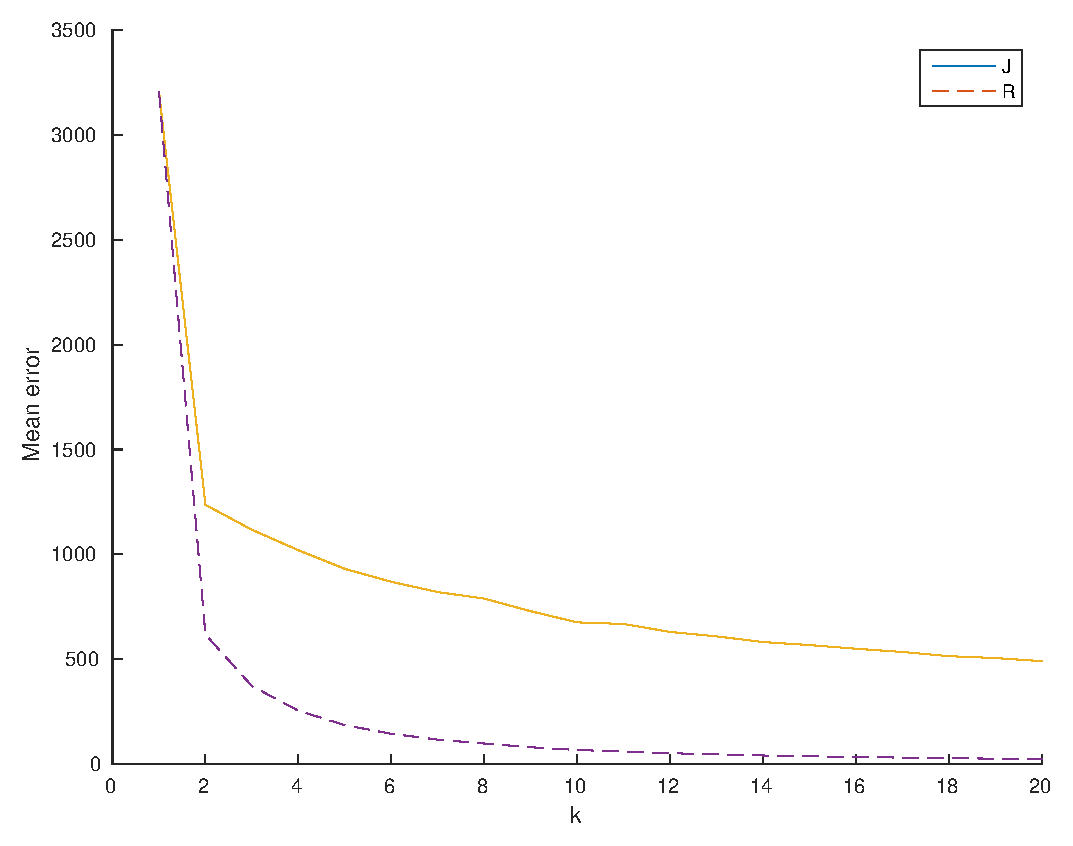
\includegraphics[width=\columnwidth]{Fig4.eps}
    \caption{The quantization error function $J(k)$ and the reference function $R(k)$.}
  \end{subfigure}
  \label{fig2.1}
\end{figure}

\section{Batch Neural gas vs k-means}

\section*{Appendix}
\lstinputlisting{../Code/kmeans.m}{\label{kmeans}}
\lstinputlisting{../Code/runKMeans.m}{\label{runKMeans}}

\end{document}
